\subsection{Results}
\label{subsec:results}

In this section, we show the results of the dynamic analysis of the structure due to the moving load, considering both cases of the initial conditions as explained in the previous section.

Again, we underline that any nodal momentum due to the moving load hasn't been taken into account in this analysis.
This might be a non-negligible approximation, but we believe that the results obtained are still meaningful for the purposes of this assignment.
Also, any inertia effects due to the acceleration of the load has been neglected.
Practically speaking then, the results here presented corresponds to a couple of purely vertical loads applied with different weights over time on the corresponding nodes in order to simulate that the mass is moving along the crane's arm.

As another example of the approximation introduced when considering a subset of mode shapes instead of the whole one, the results here presented are obtained by considering at first just the first 3 mode shapes of the structure and then the first 50 mode shapes.

\subsubsection{Initial condition 1}
\label{subsubsec:initial_condition_1}

In this case, at the start of the analysis, the structure is found in its undeformed configuration and the load is suddenly added and starts moving at $t = 0s$.

\begin{figure}[H]
    \centering
    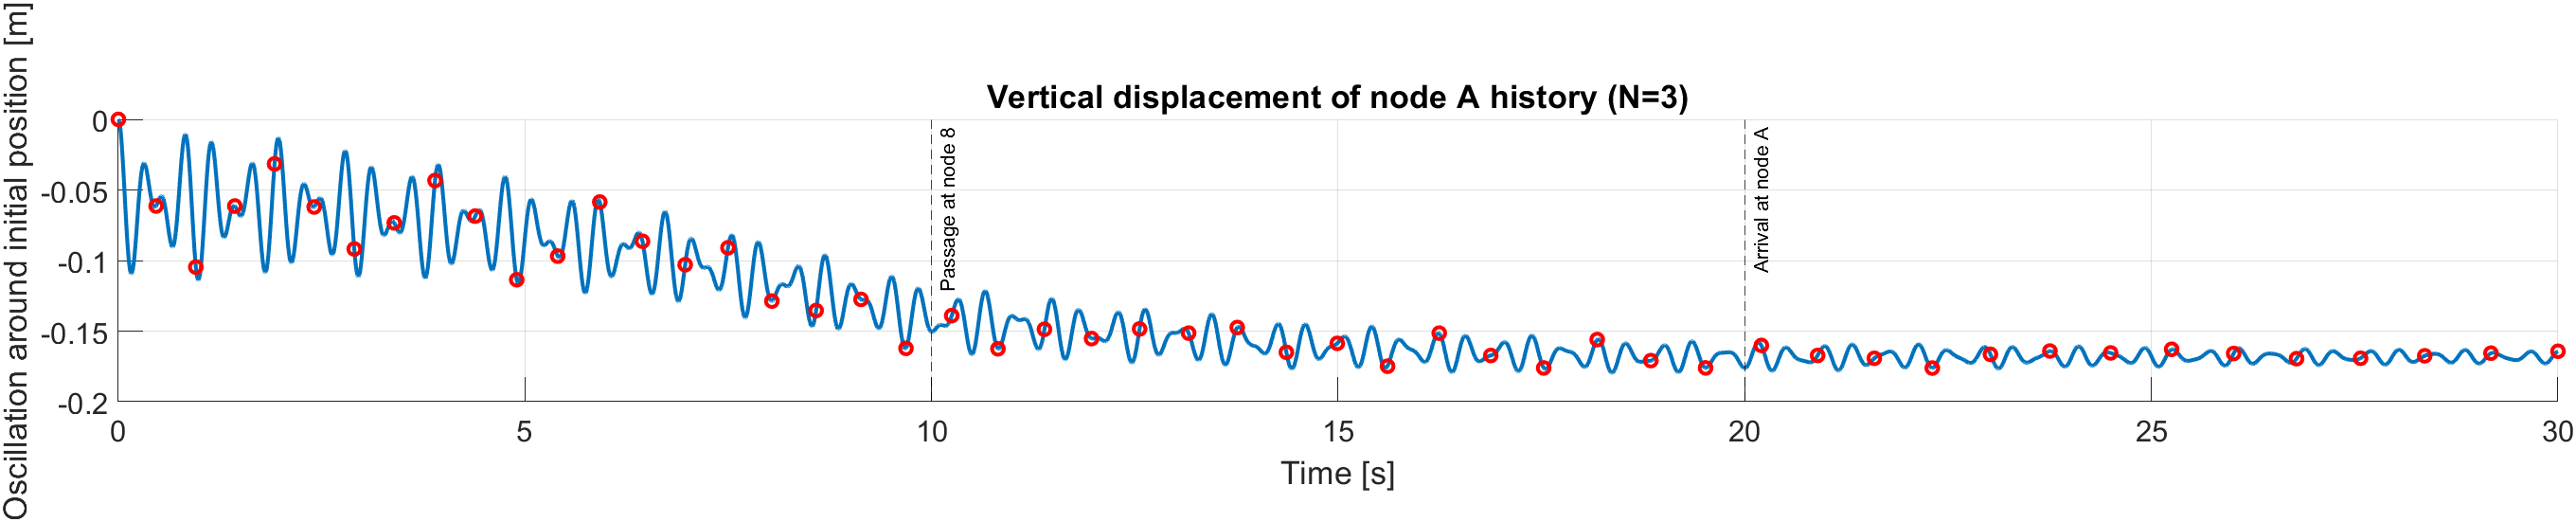
\includegraphics[width=\textwidth]{img/MATLAB/Responses/Moving_load_history_condition_1_modes_3.png}
    \caption{Dynamic response of the structure due to the moving load (initial condition 1, mode shapes considered 3).}
    \label{fig:moving_loads_response_initial_condition_1_modes_3}
\end{figure}

\begin{figure}[H]
    \centering
    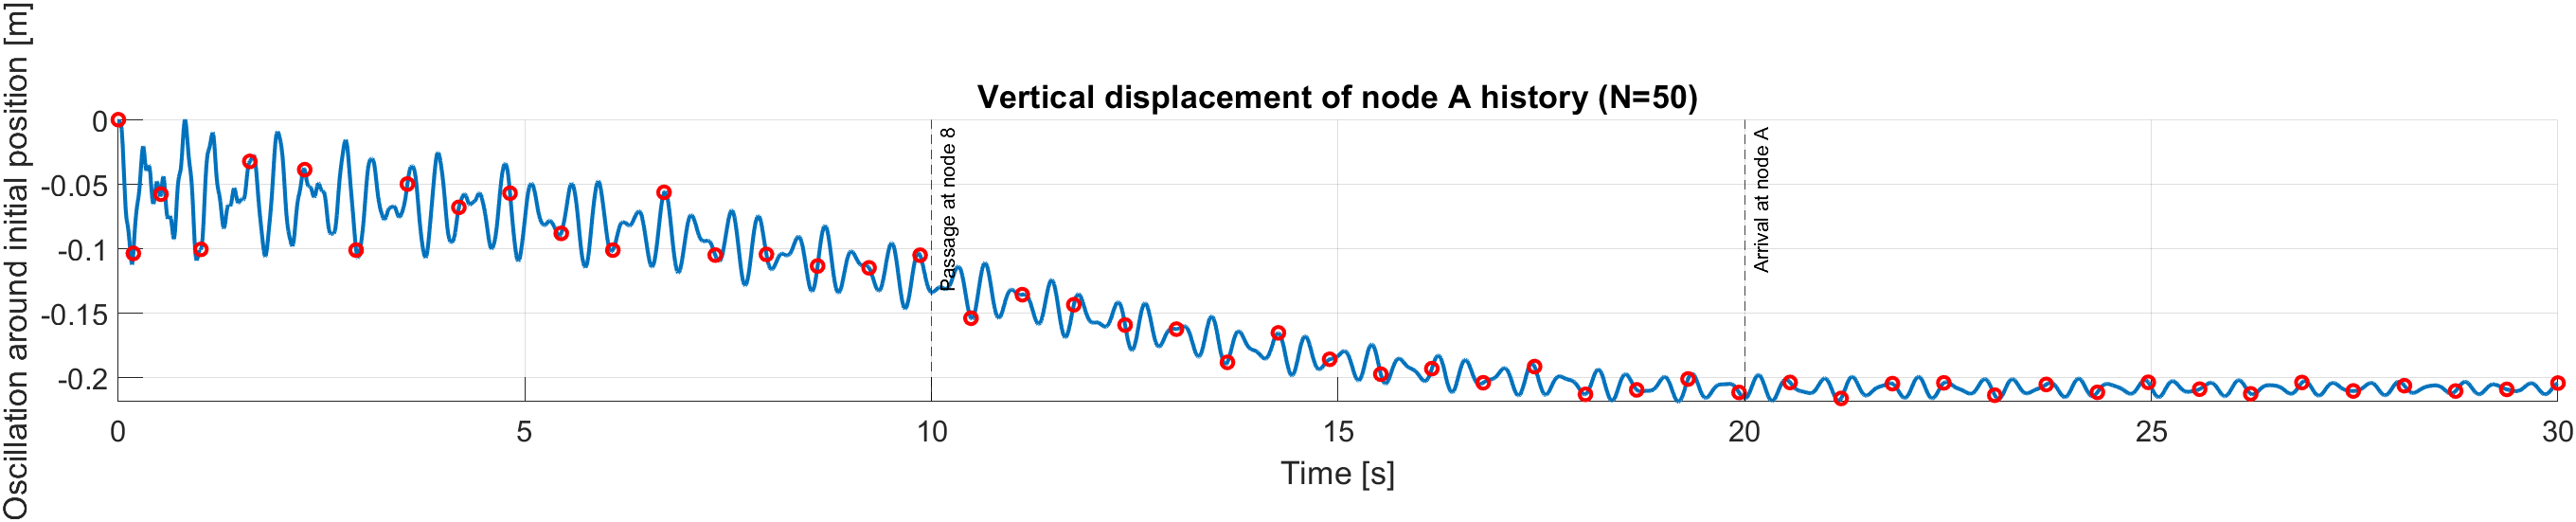
\includegraphics[width=\textwidth]{img/MATLAB/Responses/Moving_load_history_condition_1_modes_50.png}
    \caption{Dynamic response of the structure due to the moving load (initial condition 1, mode shapes considered 50).}
    \label{fig:moving_loads_response_initial_condition_1_modes_50}
\end{figure}

As we can see from the time history of node \textbf{A}, the structure shows a fast dynamic response due to the sudden addition of the load (in some sense this might be seen as a shock/impact response), overimposed to a slow dynamic response due to the moving load.

\subsubsection{Initial condition 2}
\label{subsubsec:initial_condition_2}

In this case, the structure starts from its deformed configuration due to the static loads of the mass, which then starts to move along the crane's arm at $t = 0$.

\begin{figure}[H]
    \centering
    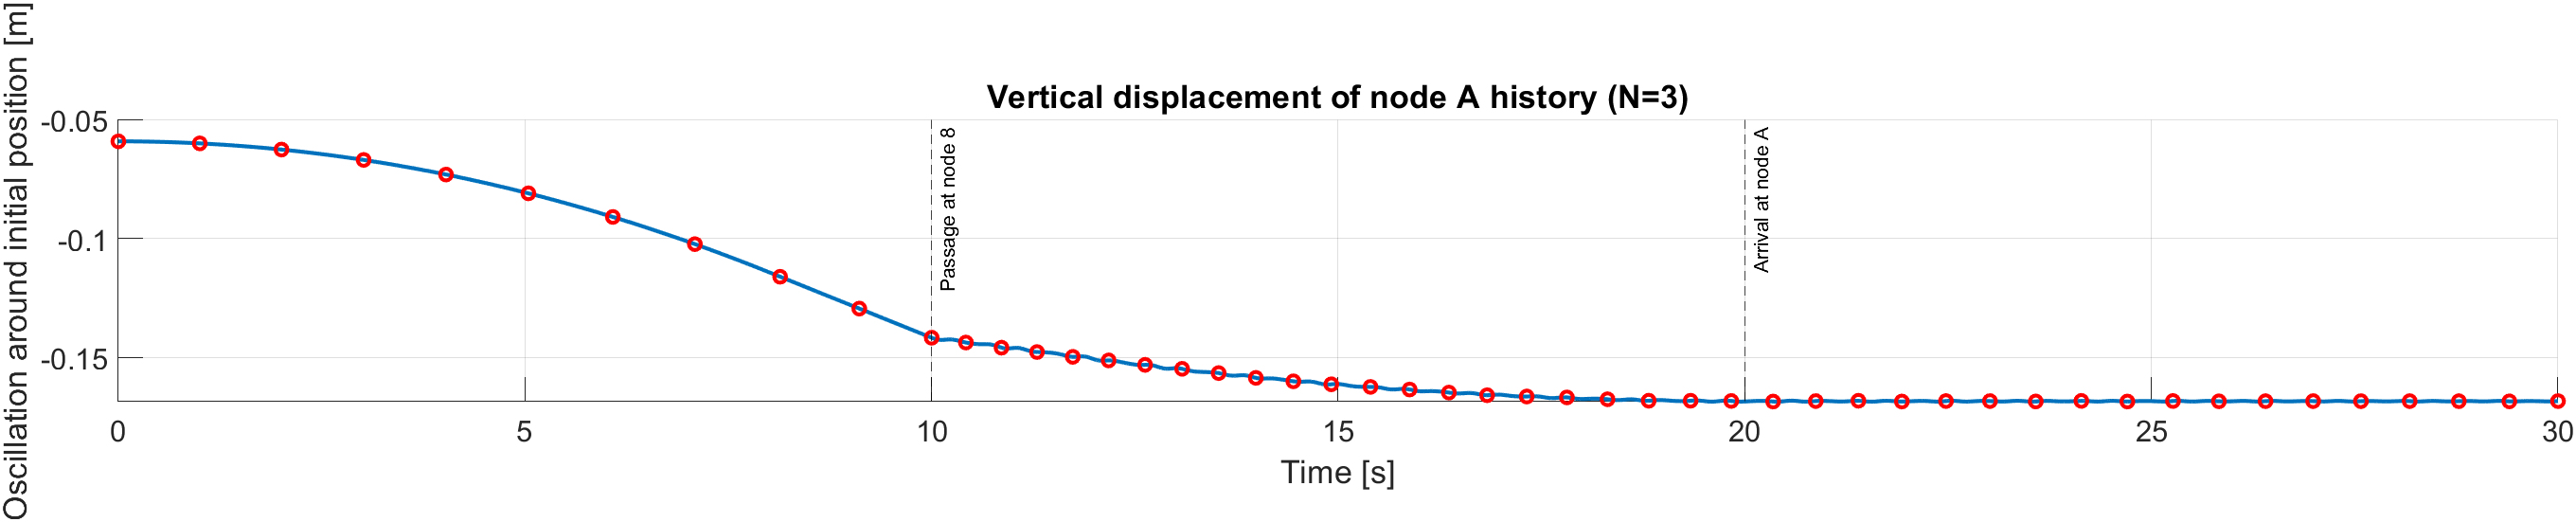
\includegraphics[width=\textwidth]{img/MATLAB/Responses/Moving_load_history_condition_2_modes_3.png}
    \caption{Dynamic response of the structure due to the moving load (initial condition 2, mode shapes considered 3).}
    \label{fig:moving_loads_response_initial_condition_2_modes_3}
\end{figure}

\begin{figure}[H]
    \centering
    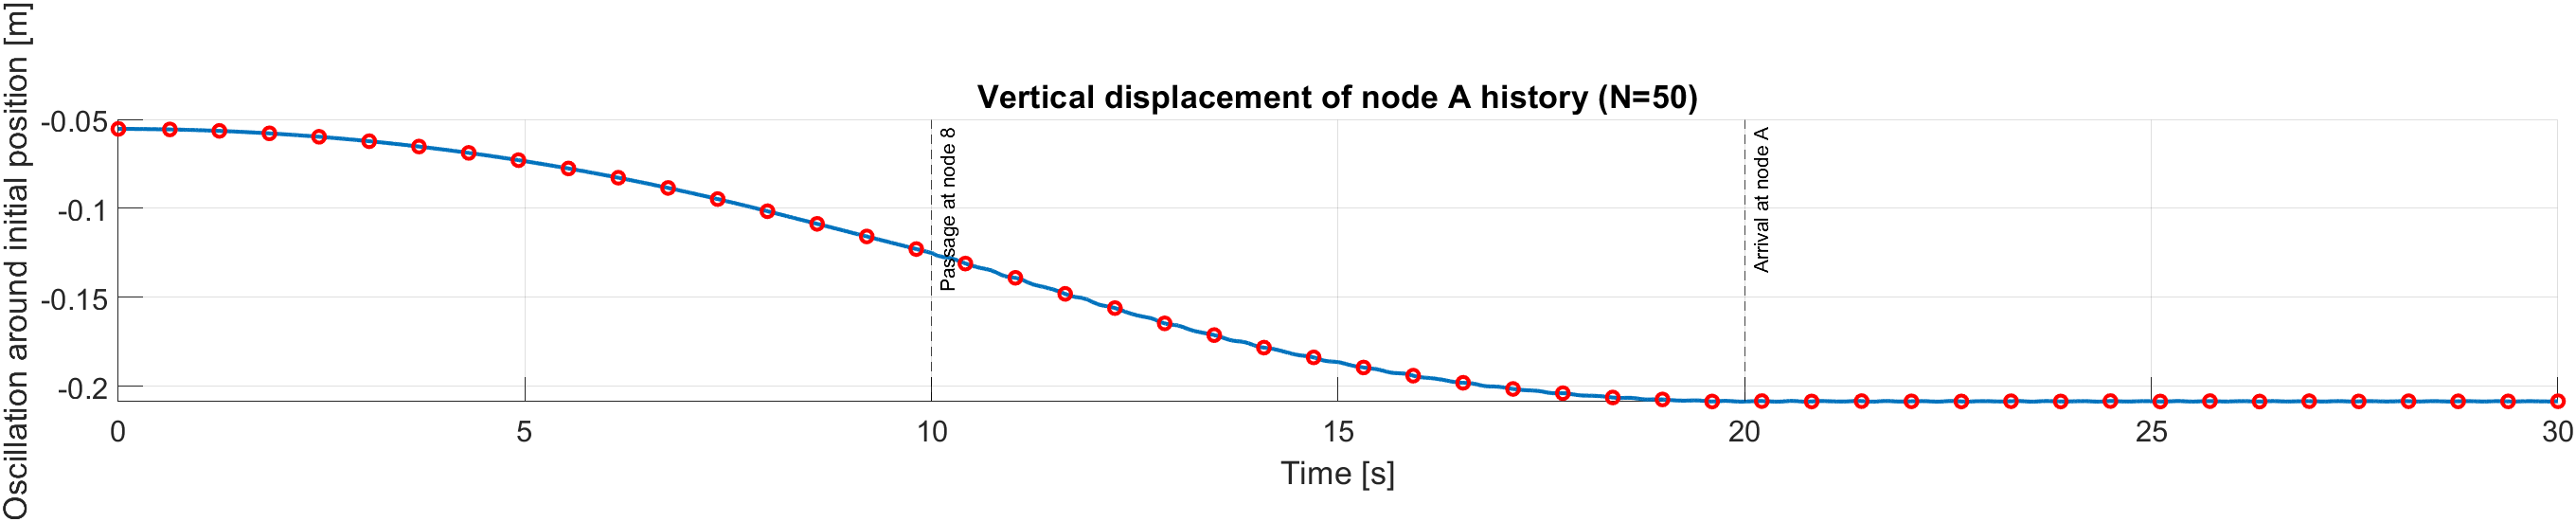
\includegraphics[width=\textwidth]{img/MATLAB/Responses/Moving_load_history_condition_2_modes_50.png}
    \caption{Dynamic response of the structure due to the moving load (initial condition 2, mode shapes considered 50).}
    \label{fig:moving_loads_response_initial_condition_2_modes_50}
\end{figure}

As we can see from the time history of node \textbf{A}, the structure shows a much more steady and controlled response, with no strong oscillatory behavior.
This can be explained by the absence of the equivalent shock/impact response due to the sudden addition of the load.